%%%%%%%%%%%%%%%%%%%%%%%%%%%%%%%%%%%%%%%%%
% Short Sectioned Assignment
% LaTeX Template
% Version 1.0 (5/5/12)
%
% This template has been downloaded from:
% http://www.LaTeXTemplates.com
%
% Original author:
% Frits Wenneker (http://www.howtotex.com)
%
% License:
% CC BY-NC-SA 3.0 (http://creativecommons.org/licenses/by-nc-sa/3.0/)
%
%%%%%%%%%%%%%%%%%%%%%%%%%%%%%%%%%%%%%%%%%

%----------------------------------------------------------------------------------------
%	PACKAGES AND OTHER DOCUMENT CONFIGURATIONS
%----------------------------------------------------------------------------------------

\documentclass[paper=a4, fontsize=11pt]{scrartcl} % A4 paper and 11pt font size

\usepackage[T1]{fontenc} % Use 8-bit encoding that has 256 glyphs
\usepackage{fourier} % Use the Adobe Utopia font for the document - comment this line to return to the LaTeX default
\usepackage[english]{babel} % English language/hyphenation
\usepackage{amsmath,amsfonts,amsthm} % Math packages

\usepackage{lipsum} % Used for inserting dummy 'Lorem ipsum' text into the template

\usepackage{sectsty} % Allows customizing section commands
\allsectionsfont{\centering \normalfont\scshape} % Make all sections centered, the default font and small caps

\usepackage{tikz}
\usetikzlibrary{plotmarks}

\usepackage{enumitem}
\usepackage{lastpage}
\usepackage{multirow}
\usepackage{fancyhdr} % Custom headers and footers
\pagestyle{fancyplain} % Makes all pages in the document conform to the custom headers and footers
\fancyhead{} % No page header - if you want one, create it in the same way as the footers below
\fancyfoot[L]{} % Empty left footer
\fancyfoot[C]{} % Empty center footer
\fancyfoot[C]{\thepage~of~\pageref{LastPage}} % Page numbering for right footer
\renewcommand{\headrulewidth}{0pt} % Remove header underlines
\renewcommand{\footrulewidth}{0pt} % Remove footer underlines
\setlength{\headheight}{13.6pt} % Customize the height of the header

\setlength\parindent{0pt} % Removes all indentation from paragraphs - comment this line for an assignment with lots of text

%----------------------------------------------------------------------------------------
%	TITLE SECTION
%----------------------------------------------------------------------------------------

\newcommand{\horrule}[1]{\rule{\linewidth}{#1}} % Create horizontal rule command with 1 argument of height



\title{	
\normalfont \normalsize 
\textsc{Norwegian University of Science and Technology\\TDT4200 -- Parallel Computing} \\ [25pt]
\horrule{0.5pt} \\[0.4cm]
\huge Problem Set 2:\\ CUDA Intro\\
\horrule{2pt} \\[0.5cm]
}

\author{Per Magnus Veierland\\permve@stud.ntnu.no}

\setlist[enumerate,1]{label=\emph{\alph*})}
\setlist[enumerate,2]{label=\roman*)}
\setlist[enumerate,3]{label=\arabic*)}

\date{\normalsize\today}

\newacro{CUDA}{Compute Unified Device Architecture}
\newacro{GPU}{Graphics Processor Unit}
\newacro{NUMA}{Nonuniform memory access}
\newacro{SGI}{Silicon Graphics International}
\newacro{SIMT}{Single Instruction Multiple Thread}
\newacro{SMT}{Simultaneous Multi-threading}
\newacro{SM}{Streaming Multi-processor}
\newacro{UMA}{Uniform memory access}

\begin{document}
\maketitle

\section*{Part 1: Theory}

\subsection*{Problem 1: Problem 1, Architectures \& Programming Models}

\begin{enumerate}

\item \textbf{Briefly explain the differences between the following architectures:\\
Keywords being: Homogeneous cores, heterogeneous cores, clusters, NUMA, threads.}

\begin{enumerate}
\item \textit{Nvidia Maxwell} is the latest generation \ac{GPU} architecture from Nvidia. Their \ac{GPU} architecture is highly parallel, with a chip such as the GM204 having 16 \acp{SM} split into 4 distinct \ac{CUDA} processing blocks, each containing 32 homogeneous \ac{CUDA} cores. In total the GM204 chip has 2048 \ac{CUDA} processing cores.

Within each \textit{processing block} (not to be mixed with \textit{thread block}) there is a register file which is shared by the processing cores and is used for thread register storage and thread local storage. All processing blocks within an \ac{SM} has one L1/texture cache as well as a shared memory. All \acp{SM} share a common L2 cache. There is no L3 cache. For each memory; the thread private memory, the \ac{SM} shared memory, and the external global memory; there is equal access time for all users, so the architecture has uniform memory access.

Threads in a \ac{CUDA} system are used to execute kernel programs. Each thread has its own program counter, registers and thread local storage. This data is stored in the processing block's register file. Threads are organized into \textit{thread blocks} by the application. The \ac{GPU} global \textit{GigaThread Engine} schedules thread blocks onto \acp{SM}. Within an \ac{SM} threads are executed as part of warps. A \textit{warp} is a collection of 32 threads which is executed simultaneously. The GM204 chip has 4 \textit{warp schedulers} per \ac{SM} which each can dispatch two instructions per warp per clock cycle. Since there is no register state within the processing cores, only in the register file, the \ac{SM} can immediately switch between executing different warps without any context switch cost. When executing a warp every processing core must execute the same instruction. This is what makes the architecture \ac{SIMT}; there is a single instruction being executed by multiple threads simultaneously. 
\item ARM big.LITTLE

\item \textit{Vilje @ NTNU} is a \ac{SGI} Altix ICE X system composed of a cluster of 1404 nodes connected by an Infiniband interconnect which is used for communication between nodes.

Each node in the system consists of two Intel Xeon ``Sandy Bridge'' processors bridged with an Intel QuickPath interconnect. Both processors has a separate 16~GB memory which they can access directly. In addition, each processor can access the memory connected to the other processor through the Intel QuickPath interconnect. This makes it a \ac{NUMA} architecture. The advantage is that each processor can access their own memory faster they would be able to access a single shared memory used by both processors; while still being able to take advantage of shared-memory programming by having access to the other processor's memory as well.

The Intel Xeon E5-2670 processors used for each node has eight homogeneous cores each for a total of 16 processing cores per node. Each processing core has a dedicated L1 (32~KB) and L2 (256~KB) cache. The L3 (20~MB) cache is shared between all cores in the processor.

The processor cores supports \ac{SMT}, also known by the term \textit{Hyper-threading} used by Intel, which allows a single physical processor core to simultaneously execute two logical threads. This is possible because each processor core is able to hold the state for two threads simultaneously and weaves their execution through a shared instruction pipeline. This technique helps the processor core better utilize all of its functional units, leading to more efficient execution.

\item Typical modern-day CPU

\end{enumerate}

\item \textbf{Explain Nvidia's SIMT addition to Flynn's Taxonomy, and how it is realized, if at all, in each of the architectures from a).}

\item \textbf{For each architecture from a), report which classification from Flynn's Taxonomy is best suited. If applicable, also state if the architecture fits Nvidia's SIMT-classification. Give the reasoning(s) behind your answers.}

\end{enumerate}

\subsection*{Problem 2: CUDA GPGPUs}

\begin{enumerate}

\item \textbf{Explain the terms \textit{Threads}, \textit{Grids}, \textit{Blocks}, and how they relate to one another (if at all).}

\begin{itemize}

\item In a \ac{CUDA} architecture a \textit{thread} represents one distinct execution of a kernel. A kernel is a general-purpose program running on the \ac{GPU} and can be executed by a large number of threads simultaneously. Each thread has its own registers, program counter and private memory. 

\item A \textit{block} is a collection of threads executing the same kernel on a single \ac{SM}. Each block has a very fast local memory which the threads within the block can use to exchange data. Blocks can be executed in any order. All threads in a block will not necessary execute at the same time; see the description of warps in the answer to question \textit{2d}. Threads in a block can synchronize their execution with a special barrier mechanism.

The \textit{number of threads per block} is specified at runtime when launching a kernel. As a convenience it is implemented as a 3-dimensional vector, where the threads for each block can be organized into 1, 2, or 3 dimensions according to what best describes the problem. The built-in variable \texttt{threadIdx} has a unique value available to each \ac{CUDA} thread specifying its \textit{X-Y-Z} index within the block. The built-in variable \texttt{blockDim} specifies the dimensions of the block.

For Maxwell, the maximum number of threads per block is $1024$, the maximum number of threads in the X-dimension for a block is $2^{32}-1$, and the maximum number of threads in the Y- and Z-dimensions is $65535$.

\item When launching a kernel, both the \textit{number of blocks} and the \textit{number of threads per block} is specified at runtime. The set of blocks instantiated for a launched kernel is known as a \textit{grid}.

The \textit{number of blocks} is also given as a 3-dimensional which can be used according to what best describes the problem. The built-in variable \texttt{blockIdx} provides the \textit{X-Y-Z} index of the block which a \ac{CUDA} thread is a part of. The built-in variable \texttt{gridDim} specifies the dimensions of the associated grid.

For Maxwell, the maximum number of blocks in the X- and Y-dimension of a grid is $1024$, and the maximum number of blocks in the Z-dimension of a grid is $64$.

\end{itemize}

Figure \ref{figure:gridblock} shows that a \textit{block} is composed of a set of \textit{threads}, that a \textit{grid} is composed of a set of \textit{blocks}, and that there is a separate \textit{grid} per \textit{kernel} executed on the \textit{device}.

\begin{figure}[p]
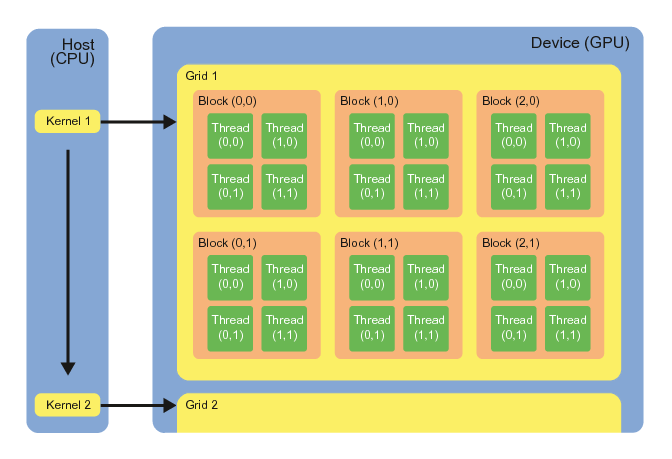
\includegraphics[width=\linewidth]{images/gridblock}
\caption{Organizational view showing how kernels, grids, blocks and threads are related in a \ac{CUDA} \ac{GPU} architecture. Source: ``Performance potential for simulating spin models on GPU'' by Martin Weigel 2011 (http://inspirehep.net/record/883697?ln=en).}
\label{figure:gridblock}
\end{figure}

%SIMT = Multiple threads execute concurrently using single instruction.
%Each thread has per-thread private local memory.
%Each thread block has per-block shared memory.
%Each grid has per-application global memory.
%
%Each thread within a thread block executes an instance of the kernel, and has a thread ID within its thread block, program counter, registers, per-thread private memory, inputs and output results.
%
%A thread block is a set of concurrently executing threads that can cooperate among themselves through barrier synchronization and shared memory. A thread block has a block ID within its grid.
%
%A grid is an array of thread blocks that execute the same kernel, read inputs from global memory, write results to global memory, and synchronize between dependent kernel calls.  
%A GPU executes one or more kernel grids; a streaming multiprocessor executes one or more thread blocks; and CUDA cores and other execution units in the SM executes threads. The SM executes threads in groups of 32 threads called a warp. Can greatly improve performance by having all threads in a warp execute same code path and access memory in nearby addresses.
%
%A CUDA core executes a floating point or integer instruction per clock for a thread. 
%
%All threads in a grid execute the same kernel function.
%
%Each thread has registers and local memory.
%
%The GigaThread global scheduler distributes thread blocks to SM thread schedulers.
%
%The SM schedules threads in groups of 32 parallel threads called warps. Each SM features two warp schedulers and two instruction dispatch units, allowing two warps to be issued and executed concurrently. 
%
%Each Streaming Multiprocessor has multiple processing cores.
%For Fermi each SM contains 32 processing cores.
%AKA ``CUDA cores''.
%These cores execute in a Single Instruction Multiple Thread fashion.
%Up to 16 SMs on a card for a maximum of 512 compute cores.
%A grid is composed of blocks which are completely independent.
%A block is composed of threads which can communicate within their own block.
%32 threads for a warp. Instructions are issued per warp. If an operand is not ready, the warp will stall. Context switching occurs between warps when stalled.
%
%Registers and shared memory are allocated for a block as long as that block is alive. Once a block is active it will stay active until all threads in that block have completed. Context switching is very fast because registers and shared memory do not need to be saved and restored.
%
%Fermi can have up to 48 active warps per SM (1536 threads).
%
%Occupancy = Active warps / Maximum active warps
%
%Occupancy can be limited by register usage. Active threads = Register memory per SM / (Registers per thread) = X threads. X threads / 1536 = occupancy
%
%Occupancy can be limited by shared memory usage: Given 48K shared memory and each kernel uses 32 bytes of shared memory per thread. 48K/32=1536 threads. Occupancy = 1
%
%Occupancy limiter: Each SM can have up to 8 active blocks. A small block size will limit the number of threads. Active threads = blockSize * maxblocks
%
%If the kernel is bandwidth bound: Attempt to increase occupancy. Use occupancy calculator.
%
%Threads can efficiently communicate and synchronize between each other; blocks cannot. Within a block, threads share data via local shared memory by using the declaration \texttt{\_\_shared\_\_} which is allocated per block. This data is not visible to threads in other blocks. Device memory is global memory. \textit{\_\_syncthreads()} can be used as a barrier to synchronize threads within a block. All threads must reach the barrier.

%__global__ is a CUDA kernel which can be called from host and from device
%__device__ is a CUDA kernel which can only be called from the device

%compute capability describes feature set of CUDA device. Number of registers, sizes of memories, features and capabilities.

%N blocks with M threads per block is launched with \texttt{kernel\textless \textlessi \textless{}N,M\textgreater \textgreater \textgreater ($\ldots$)}. Kernel launches are asynchronous.

% cudaMemcpy blocks CPU until copy is complete.
% cudaMemcpyAsync does not block CPU
% cudaDeviceSynchronize blocks CPU until all CUDA calls have completed

% blockIdx gives the block index within the grid
% threadIdx gives the grid index within the block
% blockDim gives the dimensions within each box
% gridDim gives the dimensions within the grid
% both blockIdx and threadIdx are 3-D
\item \textbf{Consider an algorithm whose input has size $2n$, output has size $5n$, and execution time is $5hn \cdot 7h \cdot \log_2(n)$ where $h = 1$ on the GPU and $h = 10$ on the CPU. The CPU-GPU bus has a bandwidth of $r$. How big must $n$ be before it is faster to run the dataset with the algorithm detailed on the GPU instead of the CPU?}

%\begin{tikzpicture}
%\draw[->] (0,0) -- (4.2,0) node[right] {$n$};
%\draw[->] (0,0) -- (0,4.2) node[above] {$T$};
%\draw[scale=0.1,domain=0:3,smooth,variable=\n,blue] plot ({\n},{5*\n*7}); % GPU
%\end{tikzpicture}

\item \textbf{Which of \texttt{kernel1()} and \texttt{kernel2()} will execute fastest, given that $X$ and $Y$ are \textit{gridDim} and \textit{blockDim} respectively, containing $3$ integers with positive powers of $2$ higher than $2^4$?}

\item \textbf{Explain each of the following terms, and how each should be utilized for maximum effect in a CUDA program:}

\begin{enumerate}
\item Warps
\item Occupancy
\item Memory Coalescing
\item Local Memory
\item Shared Memory
\end{enumerate}

\end{enumerate}

\section*{Part 2: Code}

\subsection*{Problem 1: CUDA Intro}

\begin{enumerate}

\item \textbf{In the CUDA file \texttt{lenna.cu} implement a kernel which performs the same job as the executable \texttt{cpu\_version} does. The additionally required setup of memory and variables, freeing of the same, and transfers wrt. to the CUDA kernel are also required.}

The ``Lenna'' task is to invert each pixel in a $512 \times 512$ pixel RGB-image. This task does not involve any composition of sub-results, each byte in the image needs only to be inverted once without any consideration of other pixels.

The first realization we can make is to see that the image can be seen as array of data with a size of $512 \cdot 512 \cdot 3$~bytes = $786432$~bytes and that the data does not need to be processed as individual pixels.

When building a \ac{CUDA} program from a serial program one must consider how to parallelize the program efficiently. This requires taking into account the available hardware. The hardware provided with each workstation in the Tulip lab is a \textit{GeForce GTX 750 Ti} graphics card with a Maxwell GM107 \ac{GPU}. The GM107 \ac{GPU} has 5 \acp{SM}, each with 4 distinct blocks each having an instruction buffers, warp scheduler and 32 \ac{CUDA} cores. In total the \ac{GPU} has 640 \ac{CUDA} cores.

The first idea to efficiently use the hardware was to have the largest possible number of fixed warps in execution. Using 20 warps of 32 threads all warp schedulers and \ac{CUDA} cores of the hardware should be kept active at the same time. The data is processed by 20 warps for 153 iterations, plus having the 12 first warps perform 1 extra iteration. Splitting the branching across a warp boundary should avoid warp divergence for the last iteration. The \ac{GPU} memory bus width is 128 bits and each thread will process 64 consecutive bits from memory at a time for optimal coalescence.

\begin{displaymath}
(153~\frac{\text{\footnotesize iterations}}{\text{\footnotesize thread}} \cdot 20~\text{\footnotesize warps} \cdot 32~\frac{\text{\footnotesize threads}}{\text{\footnotesize warp}} + 1~\frac{\text{\footnotesize iterations}}{\text{\footnotesize thread}} \cdot 12~\text{\footnotesize warps} \cdot 32~\frac{\text{\footnotesize threads}}{\text{\footnotesize warp}}) \cdot 8~\text{\footnotesize bytes} = 786432~\text{\footnotesize bytes}
\end{displaymath}

Averaged over 50 runs, the kernel execution time for the first approach is 40.19~us. An initial call to \texttt{cudaFree(0)} is used at the start of the program to eliminate \ac{CUDA} context initialization costs from the timing measurements.

One problem with the first approach is that the occupancy is very low. When using the \textit{CUDA Occupancy Calculator} from Nvidia the estimated occupancy of each \ac{SM} was only 17\%, given the following values:

\begin{itemize}
\item Compute capability: 2.1
\item Shared memory size: 49152 bytes
\item Threads per block: 32
\item Registers per thread: 20
\item Shared memory per block: 0
\end{itemize}

To improve upon the first attempt, a second program is written to accomplish a higher occupancy rate. Conveniently, 386 blocks with 256 threads each perfectly divides the number of bytes we wish to process by 8:

\begin{displaymath}
384~\text{\footnotesize blocks} \cdot 256~\frac{\text{\footnotesize threads}}{\text{\footnotesize block}} \cdot 8~\frac{\text{\footnotesize bytes}}{\text{\footnotesize thread}} = 786432~\text{\footnotesize bytes}
\end{displaymath}

This means that each thread only needs to calculate the complement of a single 64-bit integer. Reapplying the \textit{CUDA Occupancy Calculator} with the updated values gives an estimated occupancy of each \ac{SM} of 100\%. The averaged running time over 50 runs for the second kernel is 14.71~us.

\begin{itemize}
\item Compute capability: 2.1
\item Shared memory size: 49152 bytes
\item Threads per block: 256
\item Registers per thread: 6
\item Shared memory per block: 0
\end{itemize}

According to Nvidia the GM107 \ac{GPU} has a theoretical memory bandwidth of 86.4~GB/s (Note! $86.4 \cdot 10^6$, not $86.4 \cdot 1024^3$). The effective bandwidth utilized by the second kernel can be calculated as:

\begin{displaymath}
\textit{BW}_\text{effective} = \frac{R_B + W_B}{t_K} = \frac{2 \cdot (512 * 512 * 3\text{~bytes})}{14.71~\text{us}} = 106.92~\text{GB/s}
\end{displaymath}

Where $R_B$ is the number of bytes read from memory, $W_B$ is the number of bytes written to memory, and $t_K$ is the kernel execution time. An exact reason for why this number exceeds the theoretical bandwidth is unknown. A hypothetical kernel achieving maximum bandwidth usage should have spent 18.20~us for the given amount of data.

\textit{Reference: http://devblogs.nvidia.com/parallelforall/how-implement-performance-metrics-cuda-cc/}

\item \textbf{Implement a \texttt{make cuda} makefile rule which compiles (but does not execute) the CUDA executable \texttt{gpu\_version}.}

A \texttt{cuda} rule has been added to the provided \texttt{Makefile}.

\item \textbf{Time the transfers of data to and from device, and report the percentage of total program run-time the transfers require. How would you suggest to improve this percentage?}

After measuring the program running time it is evident that the majority of the program is spent on decoding the input image, creating the \ac{CUDA} context, and encoding the output image, see Table~\ref{table:lenna_runtime_distribution}. The measurements are a result of averaging 50 program runs. Compared to the entire program, only 0.12\% is spent on copying the input image to the device and 0.11\% is spent on copying the output image from the device.

When discounting the input image decoding, the \ac{CUDA} context initialization and the output image encoding from the consideration, the copying of the input image to the device takes 29\% of the runtime, and copying the output image from the device takes 26\% of the runtime. Whether spending more or less time of the program runtime on copying data to and from the device is ideal would depend on the problem being solved. Spending much of the runtime on copying might mean that the problem is being solved very efficiently on the \ac{GPU}. However we shall assume that it would be considered more ideal if less of the relative runtime is spent on copying and more is spent on actual computation.

Achieving this can be done by increasing the amount of data transferred to the device, and by increasing the complexity of the computation performed on the \ac{GPU}. Increasing the amount of data transferred to the device above a certain threshold will help eliminate overhead associated with the copying operation and the cost will be a more direct function of the amount of data transferred. Increasing the complexity of the computation performed will help the most by directly increasing the time of the program spent performing actual computation. For the given scenario there is no current suggestion as to how this could be achieved since the specified computation involves very cheap operations.

\begin{table}
\begin{tabular}{rrll}
Percent of program & Total time (us) & Description            & Function \\
\hline
50.8860\%          &  78228.54       & Encode output image    & \texttt{lodepng::encode} \\
37.3701\%          &  57450.24       & Create CUDA context    & \texttt{cudaFree(0)} \\
11.3247\%          &  17409.84       & Decode input image     & \texttt{lodepng::decode} \\
 0.1241\%          &    192.88       & Copy image to device   & \texttt{cudaMemcpyHostToDevice} \\
 0.1089\%          &    167.38       & Copy image from device & \texttt{cudaMemcpyDeviceToHost} \\
 0.1016\%          &    156.19       & Allocate device memory & \texttt{cudaMalloc} \\
 0.0683\%          &    104.93       & Free device memory     & \texttt{cudaFree} \\
 0.0096\%          &     14.71       & Invert pixels kernel   & \texttt{invert\_pixels} \\
\end{tabular}
\caption{Lenna program 384 blocks / 256 threads -- Runtime distribution}
\label{table:lenna_runtime_distribution}
\end{table}

\begin{figure}
\def\angle{0}
\def\radius{3}
\def\cyclelist{{"orange","blue","red","green","purple","yellow"}}
\newcount\cyclecount \cyclecount=-1
\newcount\ind \ind=-1
\begin{tikzpicture}[nodes = {font=\sffamily}]
\foreach \percent/\name in {
11.32/lodepng::decode (17.4~ms),
37.37/Initialize CUDA context (57.5~ms),
50.89/lodepng::encode (78.2~ms),
0.42/Device malloc + free + copy + kernel
} {
\ifx\percent\empty\else               % If \percent is empty, do nothing
\global\advance\cyclecount by 1     % Advance cyclecount
\global\advance\ind by 1            % Advance list index
\ifnum5<\cyclecount                 % If cyclecount is larger than list
\global\cyclecount=0              %   reset cyclecount and
\global\ind=0                     %   reset list index
\fi
\pgfmathparse{\cyclelist[\the\ind]} % Get color from cycle list
\edef\color{\pgfmathresult}         %   and store as \color
% Draw angle and set labels
\draw[fill={\color!50},draw={\color}] (0,0) -- (\angle:\radius)
arc (\angle:\angle+\percent*3.6:\radius) -- cycle;
\node at (\angle+0.5*\percent*3.6:0.7*\radius) {\percent\,\%};
\node[pin=\angle+0.5*\percent*3.6:\name]
at (\angle+0.5*\percent*3.6:\radius) {};
\pgfmathparse{\angle+\percent*3.6}  % Advance angle
\xdef\angle{\pgfmathresult}         %   and store in \angle
\fi
};
\end{tikzpicture}
\caption{Lenna program 384 blocks / 256 threads -- Total program runtime distribution}
\label{figure:lenna_total_pie}
\end{figure}

\begin{figure}
\def\angle{0}
\def\radius{3}
\def\cyclelist{{"orange","blue","red","green","purple","yellow"}}
\newcount\cyclecount \cyclecount=-1
\newcount\ind \ind=-1
\begin{tikzpicture}[nodes = {font=\sffamily}]
\foreach \percent/\name in {
24.23/cudaMalloc (156.2 us),
29.61/cudaMemcpyHostToDevice (190.9 us),
2.28/invert\_pixels (14.7 us),
25.97/cudaMemcpyDeviceToHost (167.4 us),
16.28/cudaFree (104.9 us),
1.63/Other
} {
\ifx\percent\empty\else               % If \percent is empty, do nothing
\global\advance\cyclecount by 1     % Advance cyclecount
\global\advance\ind by 1            % Advance list index
\ifnum5<\cyclecount                 % If cyclecount is larger than list
\global\cyclecount=0              %   reset cyclecount and
\global\ind=0                     %   reset list index
\fi
\pgfmathparse{\cyclelist[\the\ind]} % Get color from cycle list
\edef\color{\pgfmathresult}         %   and store as \color
% Draw angle and set labels
\draw[fill={\color!50},draw={\color}] (0,0) -- (\angle:\radius)
arc (\angle:\angle+\percent*3.6:\radius) -- cycle;
\node at (\angle+0.5*\percent*3.6:0.7*\radius) {\percent\,\%};
\node[pin=\angle+0.5*\percent*3.6:\name]
at (\angle+0.5*\percent*3.6:\radius) {};
\pgfmathparse{\angle+\percent*3.6}  % Advance angle
\xdef\angle{\pgfmathresult}         %   and store in \angle
\fi
};
\end{tikzpicture}
\caption{Lenna program 384 blocks / 256 threads -- CUDA runtime distribution}
\label{figure:lenna_cuda_pie}
\end{figure}

\end{enumerate}

\subsection*{Problem 2: Pinkfloyd Intro}

\end{document}

